\documentclass{beamer}
%\documentclass[UTF8]{ctexbeamer} % Chines Version

\usepackage[utf8]{inputenc}
\usepackage{utopia}            % font utopia imported
\usepackage{amsmath}
\usepackage{latexsym}
\usepackage{calc}              % support command '\widthof'
\usepackage{xcolor}            % support multiple color 
\usepackage{arydshln}
\usepackage{amssymb}  
\usepackage{booktabs}
\usepackage{graphicx}
\usepackage{subcaption}
\usepackage{bookmark}
\usepackage{float}
\usepackage{bm}
\usepackage{bbold}
\usepackage{extarrows}

%--------
\usepackage{listings}
\usepackage{xcolor}

\usefonttheme{professionalfonts} 

\makeatletter
\let\@@magyar@captionfix\relax
\makeatother

\usetheme{Madrid}
%\usetheme{Singapore}
%\usetheme{Pittsburgh}
%\usecolortheme{default,beaver,lily,orchid,seahorse} 
\usecolortheme{default}
%default、albatross、beaver、beetle、crane、dolphine、dove、fly、lily、orchid、rose、seagull、seahorse、sidebartab、structure、whale、wolverine

%======================================================================%
\title[CMT.SCNU]{Berry Phase And Chern Number}

%\subtitle{(To throw out a brick to attract a jade)}

\author[YuXuan Li]
{YuXuan Li\inst{1}}  

\institute[Physics@SCNU] 
{
  \inst{1}%
  Department of Physics\\
 South China Normal University 
}

\date[SCNU]{22.Dec.2020}
%======================================================================

%======================================================================
\AtBeginSection[]
{
  \begin{frame}
    \frametitle{Outline}
    \tableofcontents[currentsection]
  \end{frame} 
}
%======================================================================
 
\begin{document}
  %======================================================================
  \frame{\titlepage}
  %======================================================================

  %======================================================================
  \begin{frame}
    \frametitle{Outline}
    \tableofcontents
  \end{frame}
%======================================================================
\section{Berry Phase}
\begin{frame}
\frametitle{Berry Phase}
Berry connection is 
\begin{equation}
A(\lambda)=\langle u_\lambda|i\partial_\lambda u_\lambda\rangle=-\textrm{Im}\langle u_\lambda|\partial_\lambda u_\lambda\rangle
\end{equation}
in terms of Berry phase is 
\begin{equation}
\phi=\oint A(\lambda)d\lambda
\end{equation}
\begin{equation}
\phi=-\textrm{Im}\ln\left[\langle u_0|u_1\rangle\langle u_1|u_2\rangle\cdots\langle u_{N-1}|u_0\rangle\right]
\end{equation}
A spin-$\frac{1}{2}$ particle subjected to a uniform magnetic field $\mathbf{B}=B\hat{\mathbf{n}}$ directed along $\hat{\mathbf{n}}$
\begin{equation}
H=-\gamma \mathbf{B}\cdot \mathbf{S}=-(\frac{\gamma\hbar B}{2})\hat{\mathbf{n}}\cdot \mathbf{\sigma}
\end{equation}
\end{frame}
%----------------------------------------------------------
\begin{frame}
\frametitle{Berry Phase}
\begin{figure}
\centering
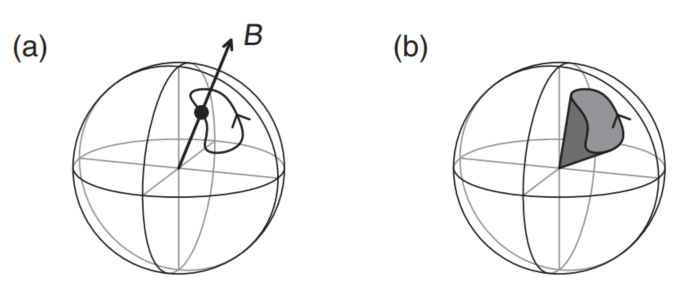
\includegraphics[scale=0.5]{pic/p1.png}
\end{figure}
\begin{equation}
\phi=-\textrm{Im}\ln\left[\langle \uparrow_z|\uparrow_x\rangle\langle\uparrow_x|\uparrow_y\rangle\langle\uparrow_y|\uparrow_z\rangle\right]
\end{equation}
\begin{equation}
|\uparrow_{\mathbf{\hat{n}}}\rangle=\left[
\begin{array}{c}
\cos(\theta/2)\\
\sin(\theta/2)e^{i\varphi}
\end{array}
\right]
\end{equation}
\begin{equation}
|\uparrow_x\rangle=\frac{1}{\sqrt{2}}\left[
\begin{array}{c}
1\\
1
\end{array}
\right]\quad
|\uparrow_y\rangle=\frac{1}{\sqrt{2}}\left[
\begin{array}{c}
1\\
i
\end{array}
\right]\quad
|\uparrow_z\rangle=\frac{1}{2}\left[
\begin{array}{c}
1\\
0
\end{array}
\right]
\end{equation}
$$\phi=\frac{\pi}{4}$$
\end{frame}
%-----------------------------------------------------
\begin{frame}
\frametitle{Berry Curvature}
\begin{equation}
A_\mu=\langle u_\lambda|i\partial_\mu u_\lambda\rangle
\end{equation}
\begin{equation}
\Omega_{\mu\nu}=\partial_\mu A_\nu-\partial_\nu A_\mu=-2\textrm{Im}\langle\partial_\mu u|\partial_\nu u\rangle
\end{equation}
\begin{equation}
\phi=\oint_P \mathbf{A}\cdot d\mathbf{\lambda}=\int_S\Omega_{\mu\nu}ds_\mu\land ds_\nu
\end{equation}
where $ds_\mu\land ds_\nu$ is an area element on the surface $S$ and $P$ is its boundary.
\begin{equation}
|\uparrow_{\hat{\mathbf{n}}}\rangle=\left[
\begin{array}{c}
\cos(\theta/2)\\
\sin(\theta/2)e^{i\varphi}
\end{array}
\right]
\end{equation}
This representation is smooth and continuous in the vicinity of "north pole"$(\theta=0)$ of the Bloch sphere. Take $\lambda=(n_x,n_y)$ through $\hat{\mathbf{n}}=(n_x,n_y,\sqrt{1-n_x^2-n_y^2})$.
\end{frame}
%-----------------------------------------------------
\begin{frame}
\frametitle{Berry Curvature}
\begin{equation}
|\uparrow_{\hat{\mathbf{n}}}\rangle\eqsim\left[
\begin{array}{c}
1\\
(n_x+in_y)/2
\end{array}
\right]\quad
|\partial_{n_x}\uparrow_{\hat{\mathbf{n}}}\rangle=\frac{1}{2}\left[
\begin{array}{c}
0\\
1
\end{array}
\right]\quad
|\partial_{n_y}\uparrow_{\hat{\mathbf{n}}}\rangle=\frac{1}{2}\left[
\begin{array}{c}
0\\
i
\end{array}
\right]
\end{equation}
$$\Omega_{xy}=-\frac{1}{2}$$
\begin{figure}
\centering
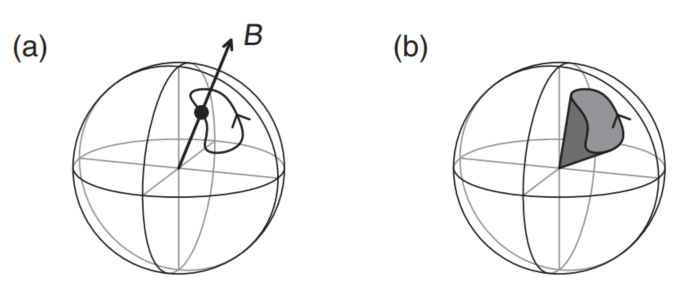
\includegraphics[scale=0.5]{pic/p1.png}
\end{figure}
\end{frame}
%======================================================
\section{Chern Theorem}
\begin{frame}
\frametitle{Chern Theorem}
\begin{figure}
\centering
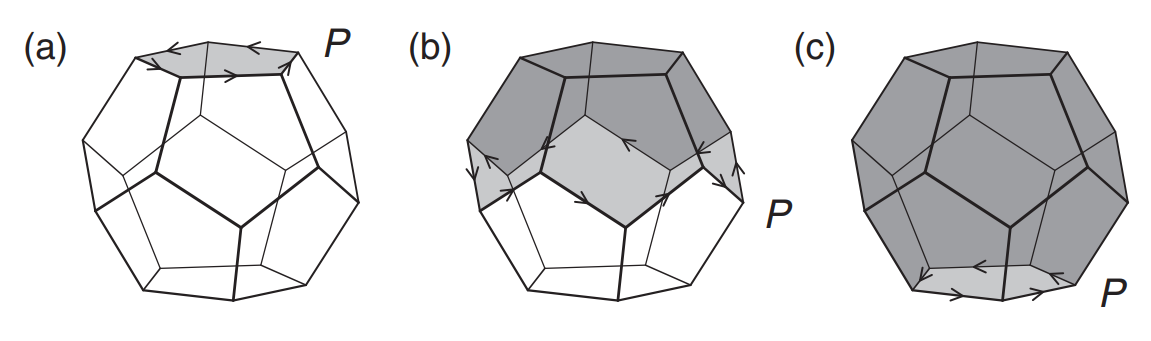
\includegraphics[scale=0.5]{pic/p2.png}
\end{figure}
$$
(a)\rightarrow-\frac{\pi}{6}\quad (b)\rightarrow-\pi\quad (c)\rightarrow-\frac{11\pi}{6}
$$
\begin{equation}
\oint_S\mathbf{\Omega}\cdot d\mathbf{S}=2\pi C
\end{equation}
\begin{block}{}
When the Chern index is nonzero, it is impossible to contruct a smooth and continuous gauage over the entire surface $S$.
\end{block}
\end{frame}
%---------------------------------------------
\begin{frame}
\frametitle{Chern Theorem}
\begin{equation}
|\uparrow_{\hat{\mathbf{n}}}\rangle=\left[
\begin{array}{c}
\cos(\theta/2)\\
\sin(\theta/2)e^{i\varphi}
\end{array}
\right]
\end{equation}
while it is smooth in the "northern hemisphere", this guage has a singularity("vortex") at $\theta=\pi$, the  "south pole".
\begin{equation}
|\uparrow_{\hat{\mathbf{n}}}\rangle=\left[
\begin{array}{c}
\cos(\theta/2)e^{-i\varphi}\\
\sin(\theta/2)
\end{array}
\right]
\end{equation}
\begin{block}{}
There is no possible choice of guage that is smooth and continuous everywhere on the unit sphere. In such a case, we say that the presence of a nonzero Chern index presents a \textcolor{red}{topological obstruction}  to the construction a globally smooth gauge.
\end{block}
\end{frame}
%-----------------------------------------------------
\begin{frame}
\frametitle{Berry Flux on a Cylinder or Torus}
\begin{figure}
\centering
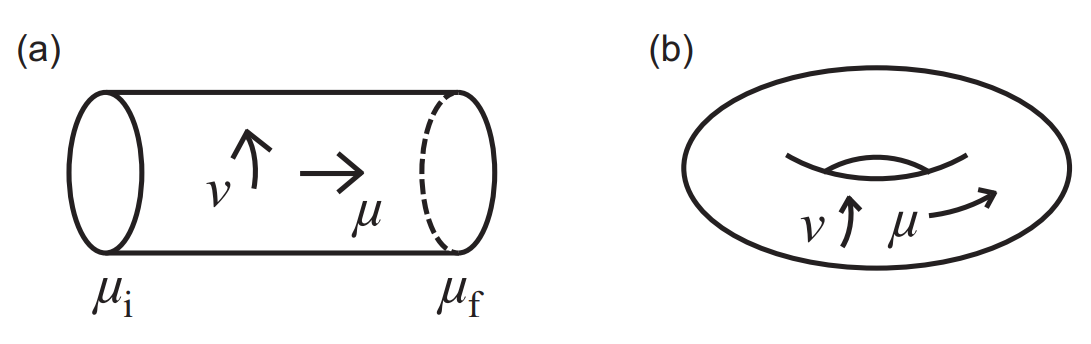
\includegraphics[scale=0.4]{pic/p3.png}
\end{figure}
Berry flux
\begin{equation}
\Phi^{\mu\nu}=\oint_S\Omega_{\mu\nu}dS
\end{equation}
For cylinder geometry
\begin{equation}
\begin{aligned}
\Phi^{\mu\nu}&=\int_{\mu_i}^{\mu_f}d\mu\int_{0}^{1}d\nu(\partial_\mu A_\nu-\partial_\nu A_\mu)\\
&=\int_{\mu_i}^{\mu_f}(\partial_\mu\phi^\nu)d\mu=\phi^\nu(\mu_f)-\phi^\nu(\mu_i)
\end{aligned}
\end{equation}
\end{frame}
%-----------------------------------------------------
\begin{frame}
\frametitle{Berry Flux on a Cylinder or Torus}
In the case $\mu=0$ and $\mu=1$ are indetified, the Berry phase at this two end points must match modulo $2\pi$. so that at the end of the crycle on the $\mu$, $\phi^\nu$ must have evolved by $2\pi m$ for some integer $m$. 
\begin{figure}
\centering
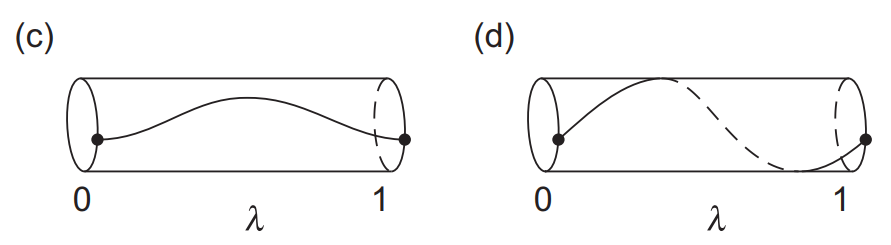
\includegraphics[scale=0.5]{pic/p4.png}
\end{figure}
\begin{block}{}
The Chern number is nothing other than the winding number of the Berry phase along $\nu$ as we evolve around a cycle in $\mu$.
\end{block}
\end{frame}
%=====================================================================================
\section{Chern Insulator}
\begin{frame}
\frametitle{Chern Insulator}
\begin{equation}
H_{CI}(\mathbf{k})=\lambda_x\sin k_x\sigma_x+\lambda_y\sin k_y\sigma_y+(m_0+t_x\cos k_x-t_y\cos k_y)\sigma_z
\end{equation}
\begin{figure}[h]
\centering
\includegraphics[scale=0.35]{pic/chernNumber.eps}
\caption{(a) Chern number of $H_{CI}$ . (b-c) Vector plot for the components $(\sin k_x,\sin k_y,(m_0+t_x\cos k_x -t_y\cos k_y))$. Common parameters:  $\lambda_x=\lambda_y=1.0,t_x=t_y=1.0$}
\end{figure}
\end{frame}
%-------------------------------------------
\begin{frame}
\frametitle{Chern Insulator}
\begin{figure}[h]
\centering
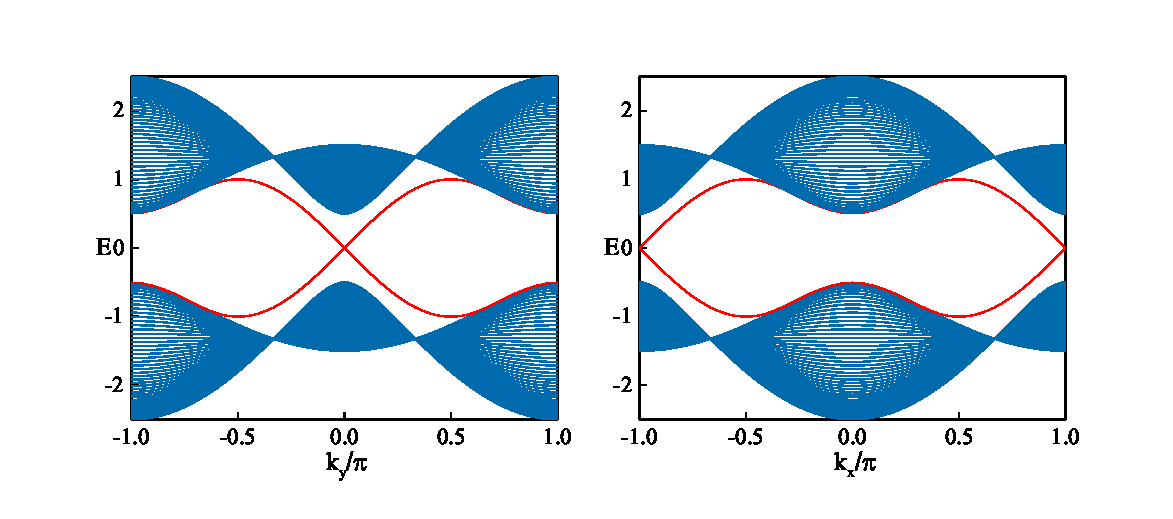
\includegraphics[scale=0.4]{pic/cy-normal.eps}
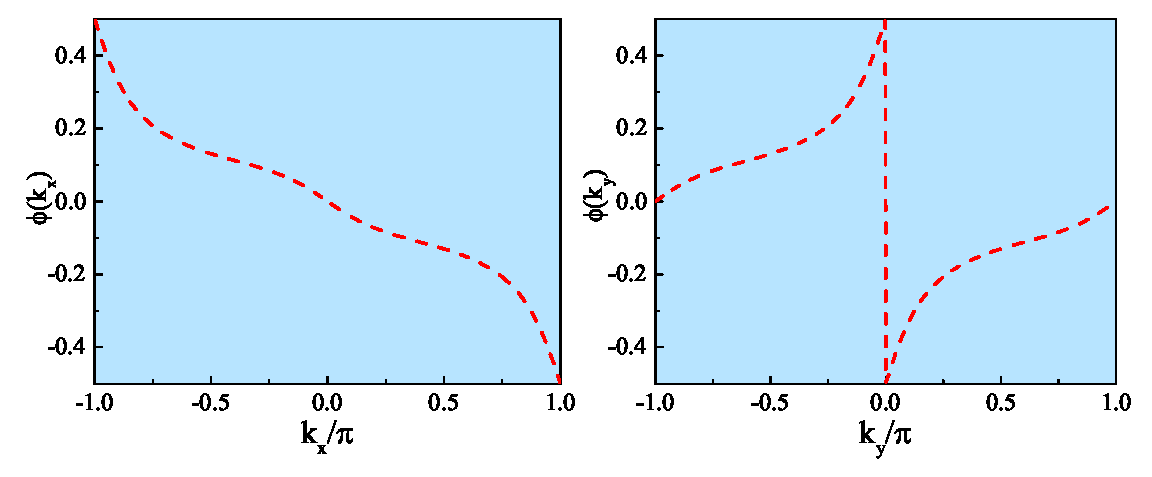
\includegraphics[scale=0.4]{pic/Berry-phase.eps}
\caption{$m_0=0.5,\lambda_x=\lambda_y=1.0,t_x=t_y=1.0$}
\end{figure}
\end{frame}





\end{document} 